\documentclass[../master_thesis_np.tex]{subfiles}
\graphicspath{ {imgs/} }


\begin{document}
	\section{Previous Developments}
	All the code work in this project is built on top of an existing code written and used in {\color{blue} MRLAB}. The existing code base was able to perform simulations of systems of active brownian particles in 2D with hard boundary, periodic or open boundary conditions featuring several confinement shapes. The only interaction which was featured in the model was a steric hard sphere correction, which is enough to study clustering and motility-induced phase separation, as well as boundary accumulation phenomena.
	
	The hardsphere correction follows the algorithm
	\begin{algorithm}[htp]
		\caption{The hard sphere correction algorithm} \label{alg:hardsphere}	
		\begin{algorithmic}[1]
			\ForAll{couples of particles $\{i, j\}$}
			\State{$d_{i,j} \gets d(\mathbf{r}_{i}, \mathbf{r}_{j})$} \Comment{$d\left(\cdot,\cdot \right)$ is the Euclidean distance}

			\State{$\mathbf{n}_{i,j} = \left(\mathbf{r}_{i}-\mathbf{r}_{j}\right)/d_{i,j}$}
			\If{$d_{i,j} < 2R$}\Comment{$R$ is the particles' radius}
			\State{$\mathbf{r}_i \gets \mathbf{r}_i - \mathbf{n}_{i,j}d_{i,j}/2$}
			\State{$\mathbf{r}_j \gets \mathbf{r}_i - \mathbf{n}_{j,i}d_{i,j}/2$}
			\EndIf
			\EndFor
		\end{algorithmic}
		\end{algorithm}
		according to \parencite{callegari_numerical_2019}.

		\begin{figure}[htp]
			\centering
			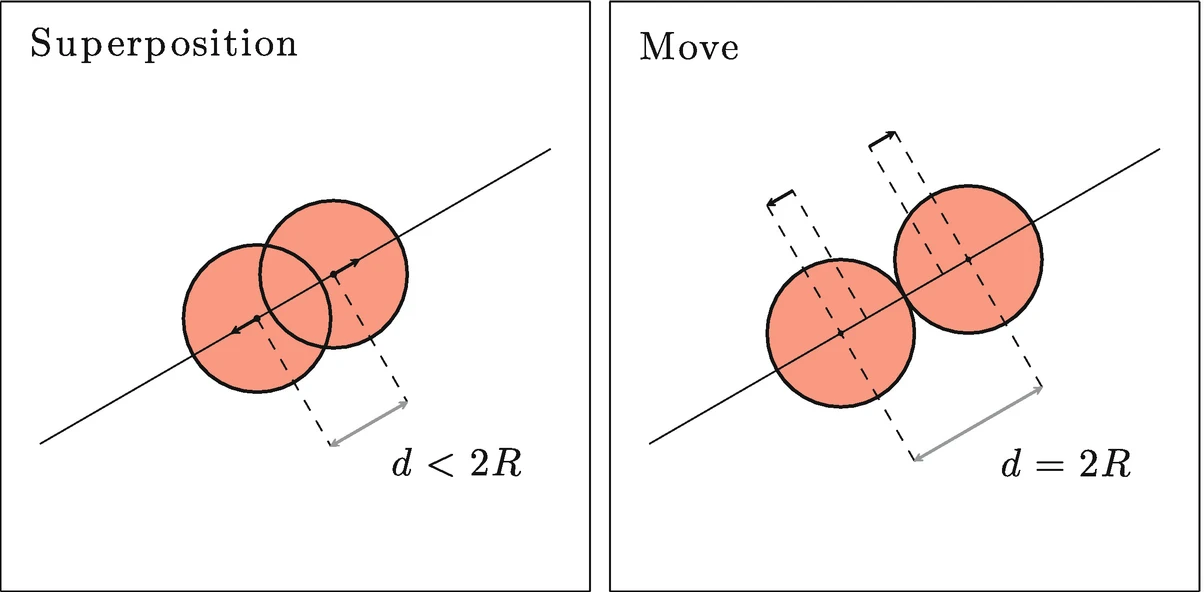
\includegraphics[width = 0.7\textwidth]{callegari_volpe_2019_hardsphere.png}
			\label{fig:hardsphere}
			\caption{{\small \fullcite{callegari_numerical_2019}}}
		\end{figure}
	\section{Steric Interactions}
	\subsection{All to All}
	\subsection{Range}
	\section{Aligning Interactions}
\end{document}